\documentclass[11pt]{standalone}
\usepackage{amssymb}
\usepackage{amsmath}
\usepackage[no-math]{fontspec}
\usepackage{unicode-math}
\usepackage{libertinus}
\usepackage{pgf,xcolor}
\usepackage{tikz}
\usetikzlibrary{arrows.meta, backgrounds}
\usepackage{pgfplots}
\pgfplotsset{compat=newest}

\definecolor{my_darkgray}{HTML}{484949}
\definecolor{my_lightgray}{HTML}{F3F4F4}
\definecolor{my_darkblue}{HTML}{005A94}
\definecolor{my_lightblue}{HTML}{CCDEE9}
\definecolor{my_yellow}{HTML}{FFEC7F}
\definecolor{my_red}{HTML}{E60000}
\definecolor{my_orange}{HTML}{E87846}

\begin{document}
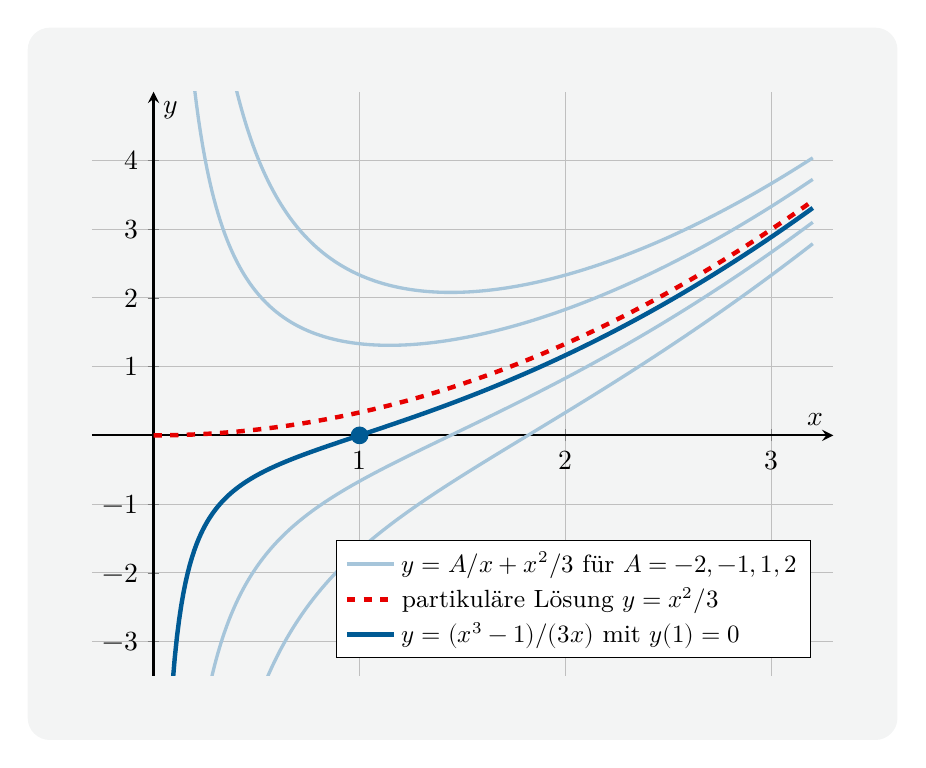
\begin{tikzpicture}[
    show background rectangle,
    background rectangle/.style={fill=my_lightgray, rounded corners=8pt},
    inner frame sep=0.8cm
]
% ---------------------------------------------------------------
%  Loesungen y = A/x + x^2/3 der DGL y' + y/x = x fuer x > 0 mit
%  A = -2, -1, 1, 2, die partikulaere Loesung y_p = x^2/3 (A = 0)
%  und hervorgehoben die Loesung des AWP y(1) = 0, also A = -1/3.
%  Werte: A = 2 bei x = 0.5, 1, 2, 3: 4.08, 2.33, 2.33, 3.67;
%         A = -2 bei denselben Stellen: -3.92, -1.67, 0.33, 2.33.
%  axis equal weggelassen: Bei gleicher Skalierung waere das Bild
%  bei y-Werten von -3.5 bis 5 und x-Werten bis 3.2 zu hoch.
% ---------------------------------------------------------------
\begin{axis}[
    axis lines = center,
    xlabel = {$x$},
    ylabel = {$y$},
    grid = both,
    axis line style={thick},
    width=11cm, height=9cm,
    xmin=-0.3, xmax=3.3,
    ymin=-3.5, ymax=5,
    xtick={1, 2, 3},
    ytick={-3, -2, -1, 1, 2, 3, 4},
    restrict y to domain=-20:20,
    legend pos=south east,
    legend style={font=\small},
    legend cell align=left,
]
\addplot[draw=my_darkblue!35, samples=300, very thick, domain=0.05:3.2]
    {2/x + x^2/3};
\addlegendentry{$y = A/x + x^2/3$ für $A = -2, -1, 1, 2$}
\foreach \A in {-2, -1, 1}{
    \addplot[draw=my_darkblue!35, samples=300, very thick, domain=0.05:3.2,
        forget plot] {\A/x + x^2/3};
}
\addplot[draw=my_red, ultra thick, dashed, samples=200, domain=0:3.2]
    {x^2/3};
\addlegendentry{partikuläre Lösung $y = x^2/3$}
\addplot[draw=my_darkblue, samples=300, ultra thick, domain=0.05:3.2]
    {x^2/3 - 1/(3*x)};
\addlegendentry{$y = (x^3 - 1)/(3x)$ mit $y(1) = 0$}
\addplot[only marks, mark=*, mark size=3pt, my_darkblue, forget plot]
    coordinates {(1, 0)};
\end{axis}
\end{tikzpicture}
\end{document}
